\documentclass[12pt,a4paper]{article}
\usepackage{float}
\usepackage{commons/course}


\hidesolutions

\شروع{نوشتار}

\سربرگ{شماره‌ی سری}{}{موضوعات تمرین}{گردآورندگان: نام افراد}


\section*{عنوان بخش}

\مسئله{سوانح هوایی}
شش پسر و نه دختر میخواهند که در یک صف کنار یکدیگر قرار بگیرند. فرض کنید متغیر S برابر با تعداد مکانهایی باشد که یک پسر و یک دختر کنار هم قرار گرفته باشند( به طور مثال در صف GBGGBBGBBGGGBGG متغیر S برابر با 8 است.)
مقدار میانگین S ( اگر تمامی ترتیب های قرار گیری این پانزده نفر را در نظر بگیریم)  برابر با چه مقداری است ؟

\حل{
	

\subsection*{الف}
		$$ 1 - \left ( \frac{5 ^ 0 e ^ {-5}}{0!} + \frac{5 ^ 1 e ^ {-5}}{1!} + \frac{5 ^ 2 e ^ {-5}}{2!} + \frac{5 ^ 3 e ^ {-5}}{3!}\right ) $$
\subsection*{ب}
		$$ 1 - (1 - e ^ {-5 \times 0.5}) = e ^ {-2.5} = 0.082$$
\subsection*{ج}
با توحه به بی حافظه بودن توزیع نمایی ، زمان پنچمین سانحه از لحظه فعلی از توزیع جمع 5 متغیر تصادفی با توزیع نمایی پیروی می کند. بنابراین  از توزیع $Gamma(5 , 5)$ پیروی می کند.کافیست مساحت زیر نمودار توزیع احتمال گفته شده را تا قبل از 0.75 بیابیم که برابر است با:
$$ 5.585808 \times 10 ^ {-7}$$ 



}


\مسئله{توزیع بتا}
\textbf{جدول
\lr{t}
در ادامه آمده است.}

اداره هواشناسی یک شهر، ۴ دستگاه سنجش آلودگی هوا را در یک منطقه قرار داده است. فرض کنید شاخص آلودگی هوا در این منطقه ثابت است اما این دستگاه‌ها دقیق نیستند و شاخص را با کمی نویز گزارش می‌دهند. در یک روز نسبتا آلوده، مقادیر گزارش شده توسط این ۴ دستگاه به شرح زیر است.
$$152, 148, 153, 153$$

\subsection*{الف}
با کمک داده‌های جمع آوری شده، یک بازه اطمینان ۹۵ درصد برای شاخص آلودگی هوا در آن ایستگاه ارائه دهید.

\subsection*{ب}
در صورتی که شاخص آلودگی هوا از ۱۵۰ بیشتر باشد، هوا در شرایط ناسالم برای تمامی گروه‌ها قرار می‌گیرد. عده‌ای از دانشمندان معتقدند که میانگین شاخص آلودگی ۱۵۰ بوده بنابراین هوای این منطقه ناسالم نیست، در حالی که عده‌ی دیگری معتقند میانگین شاخص آلودگی به طور معنی‌داری از ۱۵۰ بیشتر بوده و هوا ناسالم است. برای بررسی این افراد یک آزمون فرض طراحی کنید. فرض صفر و فرض دیگر این آزمون را بیان کرده و سپس مشخص کنید آیا با سطح اهمیت 
$0.05$
می‌توان فرض صفر را رد کرد یا خیر.

\subsection*{پ}
برای کاهش خطای نوع اول، باید سطح اهمیت را افزایش دهیم یا کاهش؟ برای کاهش خطای نوع دوم چه طور؟

\begin{figure}[H]
    \centering
    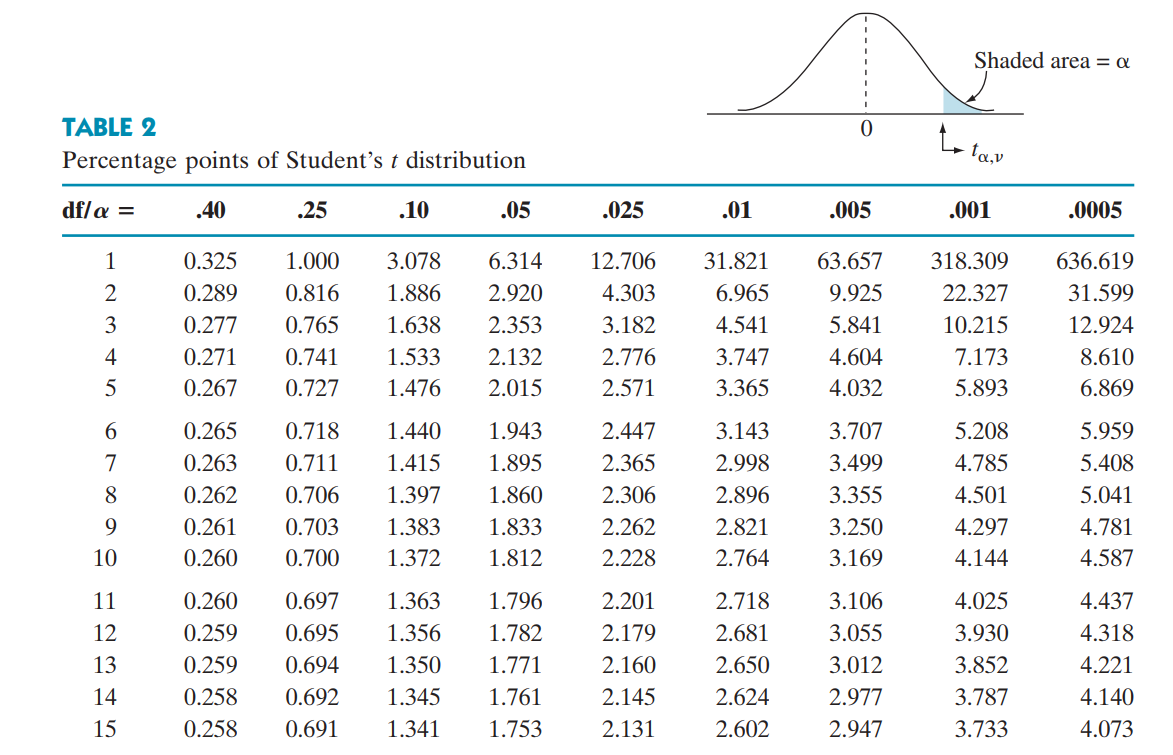
\includegraphics[width=7in,height = 5in]{tStudent}
\end{figure}

\حل{

	درست نیست ،به عنوان مثال در صورتی که:
$$S = \{1 , 2 , 3 , 4 \}$$
$$A = \{1 , 2 \} , B =  \{3 , 4 \} , C =  \{1 , 3 \} $$
داریم:
$$ P ( A \cap B ) = 0 = P ( A ) P ( B )  \Rightarrow  P ( A \cap B  | C)=0$$
$$ P (A|C)  P(B|C) = \frac{1}{4}  \Rightarrow P(A \cap B | C) \neq P(A | C) \times P(B | C)$$

}

\مسئله{چرخ بادوام}
متغیر تصادفی 
$N$
تعداد تخم مرغ های یک مزرعه است که از توزیع پوآسون با متغیر 
$\lambda$
پیروی می‌کند. هر تخم مرغ با احتمال
$p$
به جوجه تبدیل می‌شود و شکستن تخم مرغ ها از هم مستقل است . متغیر تصادفی 
$X$ 
تعداد تخم مرغ هایی هستند که به جوجه تبدیل می‌شوند و متغیر تصادفی
$Y$
 تعداد آنهایی است که تبدیل نمی‌شوند . توزیع توام را برای دو متغیر تصادفی  
$X$ و $Y$
 بدست آورید. 



\حل{
	
متغیر تصادفی $X$ را متناظر با عمر چرخ در نظر بگیرید. در نتیجه
$X \sim N(34000,4000^2)$

\subsection*{الف}
$$P(X > 40000) = 1 - P(X \leq 40000) = 1 - P(\frac{X - 34000}{4000} \leq \frac{40000 - 34000}{4000})$$
$$ = 1 - \phi(1.5) = 1 - 0.93319 = 0.06681$$
\subsection*{ب}
$$P(30000 \leq X \leq 35000) = P(\frac{30000 - 34000}{4000} \leq \frac{X - 34000}{4000} \leq \frac{35000 - 34000}{4000})$$
$$ = P(-1 \leq \frac{X - 340000}{4000} \leq 0.25) = \phi(0.25) - \phi(-1) = 0.59871 - 0.15866 = 0.44$$
\subsection*{ج}
$$P(X \geq 40000 \mid X \geq 30000) = \frac{P(X \geq 40000, X \geq 30000)}{P(X \geq 30000)} = \frac{P(X \geq 40000)}{P(X \geq 30000)}$$
$$= \frac{1 - P(\frac{X - 34000}{4000} \leq \frac{40000 - 34000}{4000})}{1 - P(\frac{X - 34000}{4000} \leq \frac{30000 - 34000}{4000})} = \frac{1 - \phi(1.5)}{1 - \phi(-1)}$$
$$ = \frac{1 - 0.93319}{1 - 0.15866} = 0.0794$$


}


\section*{عنوان بخش}

\مسئله{نقاط عجیب}
دو نفر به نام‌های A و B مشغول یک بازی هستند که شرح آن در ادامه می‌آید. ابتدا A عدد 1 یا 2 را روی یک کاغذ می‌نویسد و آن را پنهان می‌کند. B باید حدس بزند عددی که A نوشته، چه بوده است. اگر عددی که A نوشته $i$ باشد و حدس B هم درست باشد، در آن صورت A باید $i$ تومن به B بدهد. اما اگر حدس B نادرست باشد، B باید $\frac{3}{4}$ تومن به A بدهد.\\
اگر B به صورت رندوم حدس بزند به طوری که با احتمال $p$ حدس بزند 1 و با احتمال $1-p$ حدس بزند 2، امید ریاضی پول دریافتی توسط B را در دو حالت زیر محاسبه کنید.

\subsection*{الف}
اگر A عدد 1 را روی کاغذ نوشته باشد.

\subsection*{ب}
اگر A عدد 2 را روی کاغذ نوشته باشد.

\subsection*{ج}
محاسبه کنید که به ازای چه مقداری از $p$، مینیموم امید ریاضی محاسبه شده در دو حالت بالا، ماکسیموم می‌شود.

\حل{
	واقعه ی پرتاب 4ام خط شود را T4 در نظر میگیریم. 
داده های مشاهده شده یعنی 3 پرتاب اول را D در نظر میگیریم. 
پیشامد A هم این که سکه ی اولی دستمان است یا سکه ی دوم مینامیم 

بنابراین داریم:

$P(T4|D) = P(T4, A=1|D) + P(T4, A=2|D) = 
P(T4|A=1, D) \times P(A=1|D) + P(T4|A=2, D) \times P(A=2|D) = 
0.5 \times P(A=1|D) + 0.4 \times P(A=2|D)$

برای محاسبه ی $P(A=1|D)$ به این گونه عمل میکنیم:

$P(A=1|D) = \frac{P(D|A=1) \times P(A=1)}{P(D)} = \frac{P(D|A=1) \times P(A=1)}{P(D|A=1) \times P(A=1) + P(D|A=2) \times P(A=2)} = 
\frac{\frac{1}{8} \times 0.5}{\frac{1}{8} \times 0.5 + 0.144 \times 0.5} = 
\frac{0.125}{0.269} = 0.46$

بنابراین 
$P(A=2|D) = 0.54$ 
و در نتیجه داریم:

$P(T4|D) = 0.5 \times 0.46 + 0.4 \times 0.54 = 0.446$
}

\مسئله{نقطه ثابت}
صورت کلی مسئله 

\subsection*{الف}
صورت بخش اول 

\subsection*{ب}
صورت بخش دوم 

\subsection*{ج}
صورت بخش سوم

\حل{
	توضیح کلی راه حل

\subsection*{الف}
راه حل بخش اول 


\subsection*{ب}
راه حل بخش دوم 

\subsection*{ج}
راه حل بخش سوم
}

\مسئله{کشف توزیع ها}

در هر مورد تابع توزیع خواسته شده را به دست آورید و سپس تحقیق کنید متغیر تصادفی مورد نظر از چه خانواده ای از توزیع هاست. و با استفاده از آن امید ریاضی و واریانس توزیع را به دست آورید.
\subsection*{الف}
فرض کنید متغیر تصادفی $X$ از توزیع پارتو با متغیر $\theta > 0$ پیروی می کند که تابع توزیع آن به صورت زیر است:
$$f_{X}(x) = \frac{\theta}{x ^ {\theta + 1}} \quad x > 1$$
حال اگر متغیر تصادفی $Y$ به صورت زیر به دست بیاید، $Y$ از چه توزیعی پیروی می کند؟
$$ Y = \ln X$$

\subsection*{ب}
فرض کنید $Y$ متغیر تصادفی با توزیع نرمال استاندارد باشد. یعنی $Y \sim exponential(\lambda)$. حال اگر متغیر تصادفی $W$ به صورت زیر به دست بیاید، تابع توزیع آن را به دست بیاورید.$W$ از چه توزیعی پیروی می کند؟

$$W = \sqrt{Y}$$
\subsection*{ج}
فرض کنید $Z$ متغیر تصادفی با توزیع نرمال استاندارد باشد یعنی $Z \sim N(0, 1)$ . حال اگر متغیر تصادفی $Y$ به صورت زیر به دست بیاید، تابع توزیع آن را به دست بیاورید.$Y$ از چه توزیعی پیروی می کند؟
$$Z = e ^ Z$$
\subsection*{د}
فرض کنید $Z$ متغیر تصادفی با توزیع نرمال استاندارد باشد یعنی $Z \sim N(0, 1)$ . حال اگر متغیر تصادفی $X$ به صورت زیر به دست بیاید، تابع توزیع آن را به دست بیاورید.$X$ از چه توزیعی پیروی می کند؟
$$X = Z ^ 2 $$


\حل{
	

می دانیم اگر $Y = g(X)$  و ریشه های معادله $y = g(x)$ به صورت $x_1 , x_2, ...$ باشند، داریم:
$$f_{Y}(y) = \sum \frac{f_{X}(x_{i})}{|g'(x)|}$$

\subsection*{الف}
$$Y = \ln(X) \implies X = e^{Y}$$
$$f_{Y}(y) = \frac{\frac{\theta}{x^{\theta + 1}}}{\frac{1}{x}} = \theta x^{-\theta} \implies f_{Y}(y) = \theta e ^ {-y\theta}$$
پس $Y$ از توزیع نمایی با پارامتر $\theta$ است و در نتبجه :
$$ E[y] = \frac{1}{\theta}, Var(y) = \frac{1}{\theta ^ 2} $$
\subsection*{ب}
$$f_{W}(w) = \frac{\lambda e^{-\lambda y}}{\frac{1}{2 \sqrt{y}}}, y = w^{2} \implies 2w\lambda e^{-\lambda w^{2}} \sim weibull(\alpha = 2 , \beta = \frac{1}{\lambda})$$

$$E[W] = \sqrt{\beta} \times \Gamma (1 + \frac{1}{\alpha}) = \frac{1}{\sqrt{\lambda}}\Gamma (\frac{3}{2})$$
$$Var[W] = \beta[\Gamma(1 + \frac{2}{\alpha}) - (\Gamma(1 + \frac{1}{\alpha})) ^ {2}] = \frac{1}{\lambda}[\Gamma(2) - (\Gamma(\frac{3}{2})) ^ {2}]$$
\subsection*{ج}
$$f_{X}(x) = \frac{\frac{1}{\sqrt{2\pi}}e^{\frac{-z^2}{2}}}{e^{z}} = \frac{1}{\sqrt{2\pi}}e^{-\frac{(\ln x) ^ 2}{2}} \sim lognormal(\mu = 0, \sigma ^ 2 = 1)$$
$$E[x] = exp(\mu + \frac{\sigma ^ 2}{2}) = e ^ {\frac{1}{2}}$$
$$Var[x] = [exp(\sigma ^ 2) - 1]exp(2\mu + \sigma ^ 2) = e^2 - e$$
\subsection*{د}
$$x = z ^ 2 \implies z_{1} = \sqrt{x}, z_{2} = -\sqrt{x}$$
$$f_{X}(x) = \sum \frac{\frac{1}{\sqrt{2\pi}}e ^ {\frac{-z_{i} ^ 2}{2}}}{2|z_{i}|} = 2 \times \frac{1}{2\sqrt{2\pi x}}e ^ {\frac{-x}{2}} = \frac{1}{\sqrt{2 \pi x}}x ^ {-\frac{1}{2}}e ^ {-\frac{x}{2}} \sim gamma(k = \frac{1}{2} , \theta = 2)$$
$$E[X] = k\theta  = 1$$
$$Var[X] = k\theta ^ 2 = 2$$
دقت کنید که به طور کلی نیازی به در نظر گرفتن ضرایب ثابت در توزیع ها وجود ندازد ، چرا که نهایتا جمع(انتگرال) تابع توزیع چگالی برابر یک خواهد بود.

}

\مسئله{روابط}

تعداد زیرمجموعه های k عضوی از مجموعه ی $\{1, 2, 3, ..., n\}$ را بیابید که هیچ دو عضوی از آن متوالی نباشند.


\حل{
	\subsection*{الف}
$$E[X] = \sum_{i = 1}^{\infty} i P(X = i)$$
$$ = P(X = 1)$$
$$ + P(X = 2) + P(X = 1)$$
$$ + P(X = 3) + P(X = 2) + P(X = 1)$$
$$ . . .$$
حالا اگر به صورت ستونی جمع بزنیم(یعنی حاصل جمع ستون ها را در نظر بگیریم) ، تساوی بالا به دست می آید.
\subsection*{ب}
می دانیم که
$$F_X(x) = P(X \leq x) \implies 1 - F_X(x) = P(X > x)$$
در نتیجه:
$$\int_{0}^{\infty} (1-F_X(x))\,dx = \int_0^\infty P(X> x) dx = \int_0^\infty \int_x^\infty f_X(y) dy dx$$
$$= \int_{0< x< y< \infty} f_X(y) d (x,y) = \int_0^\infty \int_0^y f_X(y) dx dy$$
از طرفی می دانیم:
$$\int_0^y f_X(y)\operatorname d x = f_X(y) \int_0^y 1\operatorname d x = y~f_X(y)$$
بنابراین:
$$\int_0^\infty P(X> x)dx = \int_0^\infty yf_X(y) dy = E(X \mid X\geq 0)P(X\geq 0) = E[X]$$ 
در صورتی که $X$ همواره مثبت باشد.


}

\مسئله{ظرف گوی}
ثابت کنید متغیرهای
$ X_1 $
, ... ,
$ X_n $
مستقلند اگر و تنها اگر تابع توزیع توام آن‌ها به شکل زیر قابل بیان باشد.
\begin{center}
	$f( x_1, x_2, ..., x_n ) = \prod_{i=1}^n g_i(x_i)$
\end{center}
$ g_i $
تابعی مثبت است.

\حل{
	با استفاده از استقرا قابل است که:
\begin{center}
	$ \int_{-\infty}^{\infty} g_i(x_i) dx_i = 1$
\end{center}
.
برای اثبات حکم روی
$ n $
استقرا میزنیم.
\\
پایه استقرا: برای
$ n = 2 $
میدانیم، اگر
$ x_1 $
و
$ x_2 $
مستقل باشند، آنگاه؛
\begin{center}
	$ f(x_1, x_2) = f_1(x_1) f_2(x_2) $
\end{center}
است. در نتیجه توزیع توام این دو متغیر به شکل 
$ g_1(x_1) g_2(x_2) $
قابل بیان است.
\\
همچنین اگر 
$ f(x_1, x_2) = g_1(x_1) g_2(x_2) $
داریم:
\begin{center}
	$ f_2(x_2) = \int_{-\infty}^{\infty} f(x_1, x_2) dx_1 = \int_{-\infty}^{\infty} g_2(x_2) g_1(x_1) dx_1 = g_2(x_2)$
	\\
	$ f_1(x_1) = \int_{-\infty}^{\infty} f(x_1, x_2) dx_2 = \int_{-\infty}^{\infty} g_1(x_1) g_2(x_2) dx_2 = g_1(x_1)$
	\\
	$ \rightarrow f(x_1, x_2) = g_1(x_1) g_2(x_2) = f_1(x_1) f_2(x_2)$
\end{center}
بنابراین دو متغیر 
$ x_1 $
و
$ x_2 $
مستقلند.
گام استقرا:
فرض کنید متغیرهای
$ x_1,..., x_n, x_{n+1} $
از یکدیگر مستقل باشند.
حال با توجه به فرض استقرا؛
\begin{center}
	$ f(x_1,..., x_n | x_{n+1}) = f(x_1,..., x_n) f_{n+1}(x_{n+1}) = \prod_{i=1}^{n} g_i(x_i) f_{n+1}(x_{n+1})$
\end{center}
همانطور که مشاهده شد فرم مذکور در صورت سوال قابل مشاهده است.
\\
حال فرض میکنیم،
$ f(x_1,..., x_n, x_{n+1}) = \prod_{i=1}^{n+1} g_i(x_i) $
است.
\\
با انتگرالگیری روی 
$ x_{n+1} $
داریم:
\begin{center}
	$ f(x_1,..., x_n) = \prod_{i=1}^{n} g_i(x_i) $
\end{center}
باتوجه به فرض استقرا متغیرهای
$ x_1,..., x_n $
از یکدیگر مستقلند. میتوان معادله‌ی بالا را فرم زیر نوشت.
\begin{center}
	$ f(x_1,..., x_n, x_{n+1}) = f(x_1,..., x_n) g_{n+1}(x_{n+1}) $
\end{center}
با انتگرالگیری روی
$ x_1 $
تا
$ x_n $
نتیجه میشود:
\begin{center}
	$ f_{n+1}(x_{n+1}) = \int_{-\infty}^{\infty} ... \int_{-\infty}^{\infty} f(x_1,..., x_n, x_{n+1}) dx_1 ... dx_n = g_{n+1}(x_{n+1}) $
	\\
	$ \rightarrow f(x_1,..., x_n, x_{n+1}) = f(x_1,..., x_n) f_{n+1}(x_{n+1}) $
\end{center}
در نتیجه متغیرهای مستقلند.
}

\مسئله{فلامینگو توانا}
در یک جعبه m توپ قرمز و n توپ آبی داریم.در هر مرحله یک توپ را به تصادف از جعبه خارج میکنیم تا زمانی که در مجموع r توپ قرمز دیده باشیم. احتمال این که در مجموع k توپ از جعبه بیرون آورده باشیم چه قدر است؟ 


\حل{
	در حالت کلی برای انتخاب سه نفر از هفت نفر \(\binom{7}{3}\) راه داریم. حال از این تعداد حالاتی را که حداقل دو نفر از سه نفر انتخاب شده کنار هم باشند را محاسبه می کنیم. برای این کار ابتدا تعداد حالاتی را که هیچ دو نفری کنار هم نیستند را به دست آورده و سپس با بهره گیری از اصل متمم به حل سوال میپردازیم. با کمی دقت درمیابیم که به ازای هر انتخاب برای نفر اول، سه انتخاب برای دو نفر دیگر داریم.از طرفی هر حالت سه بار شمرده می شود.\\
برای انتخاب سه نفر که هیچ یک کنار یکدیگر نباشند 
\(\frac{7 \times 3}{3} = 7\)
حالت داریم.
پس\\ خواهیم داشت : 
 \(\frac{4}{5}\)\) = \(1 - \frac{7}{\(\binom{7}{3}\)} 
}

\مسئله{پرواز خطرناک}
فرض کنید متغیر تصادفی X از یک توزیع
$
Binomial(n, p)
$
می‌آید.
\subsection*{الف}
با فرض اینکه 
$
p < \alpha < 1
$
و استفاده از نابرابری چبیشف، یک کران بالا برای 
$
P(X \ge \alpha n)
$
بیابید.

\subsection*{ب}
مقدار کران بالا را برای 
$
p = \frac{1}{2}
$
و
$
\alpha = \frac{3}{4}
$ 
تعیین کنید.


\حل{
	\subsection*{الف}
می‌توانیم برای محاسبه کران بالا بنویسیم:
\begin{align*}
P(X \ge \alpha n) &= P(X - np \ge \alpha n - np) \\
&\le P(|X - np| \ge n \alpha - np) \\
&\le \frac{Var(X)}{(n\alpha - np)^2} \\
&= \frac{p(1 - p)}{n(\alpha - p)^2} \\
\end{align*}
\subsection*{ب}
با جایگذاری 
$
p = \frac{1}{2}
$
و 
$
\alpha = \frac{3}{4}
$
داریم:
$$
P(X \ge \frac{3n}{4}) \le \frac{4}{n}
$$

}

\مسئله{استاد حواس پرت}

استاد حواس پرتی را در نظر بگیرید که برای دو دانشجو در زمان یکسان قرار ملاقات می گذارد.اما متاسفانه استاد در هر زمان فقط می تواند با یک دانشجو ملاقات کند.مدت زمان ملاقات دو دانشجو مستقل از یکدیگر و دارای توزیع نمایی با میانگین 30 دقیقه است.امید ریاضی فاصله زمانی بین ورود دانشجوی اول و خروج دانشجوی دوم را در دو حالت زیر بیابید.
\subsection*{الف}
دانشجوی اول سر وقت حاضر می شود ولی دانشجوی دوم 5 دقیقه دیر میرسد.(تذکر:جواب 60 دقیقه یا 65 دقیقه نیست)
\subsection*{ب}
دانشجوی اول سر وقت حاضر می شود ولی دانشجوی دوم $X$ دقیقه دیر میرسد که $X$ دارای توزیع نمایی با میانگین 5 دقیقه است.



\حل{
	طبق نابرابری مارکوف داریم:
$$
P(X \ge 49) \le \frac{E(X)}{49}
$$
از طرفی،
$$
P(X \ge 49) \ge \frac{99}{100}
$$
پس
\begin{align*}
&\frac{E(X)}{49} \ge \frac{99}{100}\\
&\Rightarrow \frac{N\frac{98}{100}}{49} \ge \frac{99}{100} \\
&\Rightarrow \frac{2N}{100} \ge \frac{99}{100} \\
& \Rightarrow N \ge 50
\end{align*}

بنابراین حداقل 50 قطعه RAM باید خریداری شود.

}

\مسئله{مغازه خالی}

فرض کنید زمان بین آمدن دو مشتری در یک مغازه از توزیع نمایی با پارامتر $\lambda$  و میانگین 2 دقیقه پیروی می کند.فرض کنید شما از جلوی مغازه رد می شوید و میبیند که مغازه خالی است.به چه احتمالی تا 5 دقیقه دیگر این مغازه خالی می ماند؟


\حل{
	
می دانیم که $E[x] = \frac{1}{\lambda}$ چون نوزیع $X$ توانی با پارمتر $\lambda$ است و از طرفی گفته شده است که میانگین 2 دقیقه است پس $\lambda = 0.5 min $ می باشد.فرض کنید در لحظه $t$ از جلوی مغازه می گذریم و میبینم که خالی است.مسئله از ما میخواد تا مقدار زیر را محاسبه کنیم:
$$P(X > t + 5 | X > t)$$ 
اما می دانیم که توزیع $X$ نمایی است و این توزیع بی حافظه است در نتیحه مقدار بالا برابر است با :
$$P(X > 5) = e ^ {-\lambda 5} = e ^ {- \frac{5}{2}}$$
}


\begin{flushleft}
	موفق باشید :)
\end{flushleft}



\پایان{نوشتار}
